\documentclass[12pt, a4paper]{article}


% **************************************
% *            中文字体设置              *
% **************************************
\usepackage{xeCJK}
\usepackage[UTF8]{ctex}
\setmainfont{Times New Roman}
\setCJKmainfont{宋体}

\setCJKfamilyfont{zhhei}{黑体}
\newcommand*{\hei}{\CJKfamily{zhhei}}
\setCJKfamilyfont{zhkai}{楷体}
\newcommand*{\kai}{\CJKfamily{zhkai}}
\setCJKfamilyfont{enroman}{Times New Roman}
\newcommand*{\mytimes}{\CJKfamily{enroman}}

% **************************************
% *            页面设置                 *
% **************************************
\usepackage[left=2.0cm, right=2.0cm, top=2.0cm, bottom=2.0cm]{geometry} %设置页边距的宏包

\usepackage{graphicx} %插入图片的宏包
%\graphicspath{{chapter/}{figures/}}
\usepackage{indentfirst} %自动缩进
\usepackage{xcolor} %语法高亮支持
\usepackage{float} %可以用于禁止浮动体浮动
\usepackage{subfigure} %插入多图时用子图显示的宏包

\usepackage[colorlinks,linkcolor=black,anchorcolor=blue,citecolor=black]{hyperref}
\hypersetup{hidelinks} %隐藏超链接上的外框
%\usepackage[colorlinks,linkcolor=red]{hyperref}%超链接

\usepackage{fontspec,xltxtra,xunicode}
\defaultfontfeatures{Mapping=tex-text} %如果没有它,会有一些 tex 特殊字符无法正常使用,比如连字符
% 文章内中文自动换行,可以自行调节
\XeTeXlinebreaklocale “zh”
\XeTeXlinebreakskip = 0pt plus 1pt minus 0.1pt

% 下面的命令设置行间距与段落间距
\linespread{1.4}
% \setlength{\parskip}{1ex}
\setlength{\parskip}{0.5\baselineskip}

\usepackage{fancyhdr} %使用fancyhdr包自定义页眉页脚
%\pagestyle{empty}
\pagestyle{fancy}
%\pagestyle{plain} %没有页眉,页脚放页数
\renewcommand{\headrulewidth}{0.5pt}
\renewcommand{\footrulewidth}{0.4pt}
\lhead{}
\chead{}
\rhead{}
\lfoot{}
\cfoot{\thepage}
\rfoot{}
\usepackage{booktabs} %表格用


\usepackage{listings} %可以插入代码
%代码格式
\definecolor{dkgreen}{rgb}{0,0.6,0}
\definecolor{gray}{rgb}{0.5,0.5,0.5}
\definecolor{mauve}{rgb}{0.58,0,0.82}
\lstset{ %
	%	language=Python,                % the language of the code
	breaklines, %自动折行
	%extendedchars=false %解决代码跨页时,章节标题,页眉等汉字不显示的问题
	keepspaces=false,
	%tabsize=4 %设置tab空格数
	showspaces=false, %不显示空格
	showtabs=false,
	showstringspaces=true,
	numbers=left,
	basicstyle=\footnotesize,
	numberstyle=\tiny,
	numbersep=5pt,
	keywordstyle= \color{ blue!70}, %关键字颜色
	commentstyle= \color{red!50!green!50!blue!50}, %注释颜色 
	frame=shadowbox, %边框格式:阴影效果
	rulesepcolor= \color{ red!20!green!20!blue!20},
	escapeinside=``, %英文分号中可写入中文
	xleftmargin=2em,xrightmargin=2em, aboveskip=1em,  %设置页边距
	framexleftmargin=2em
}

\makeatletter
\renewcommand\abstract{%
\kai\textbf{\hei{摘要:}}
{\normalfont\xiaosihao\kai}}
\makeatother

\newenvironment{enabstract}

\makeatletter
\renewcommand\enabstract{%
\textbf{Abstract: }
{\normalfont\xiaosihao\mytimes}}
\makeatother

%%%% 设置 key words 属性 %%%%
\newenvironment{keys}

\makeatletter
\renewcommand\keys{%
\kai\textbf{\hei{关键词:}}
{\normalfont\xiaosihao\hei}}
\makeatother

\newenvironment{enkeys}

\makeatletter
\renewcommand\enkeys{%
\textbf{Key words: }
{\normalfont\xiaosihao\mytimes}}
\makeatother

% **************************************
% *      数学符号                       *
% **************************************
\usepackage{amsmath,amssymb}
\usepackage{bm} % $\bm{letter}$ 数学式中粗斜体字母的最佳方案
\usepackage{calc}
\usepackage{units} %单位宏包

% **************************************
% *     定义中文字号                     *
% **************************************
\newcommand{\chuhao}{\fontsize{42pt}{\baselineskip}\selectfont}
\newcommand{\xiaochuhao}{\fontsize{36pt}{\baselineskip}\selectfont}
\newcommand{\yihao}{\fontsize{28pt}{\baselineskip}\selectfont}
\newcommand{\erhao}{\fontsize{21pt}{\baselineskip}\selectfont}
\newcommand{\xiaoerhao}{\fontsize{18pt}{\baselineskip}\selectfont}
\newcommand{\sanhao}{\fontsize{15.75pt}{\baselineskip}\selectfont}
\newcommand{\sihao}{\fontsize{14pt}{\baselineskip}\selectfont}
\newcommand{\xiaosihao}{\fontsize{12pt}{\baselineskip}\selectfont}
\newcommand{\wuhao}{\fontsize{10.5pt}{\baselineskip}\selectfont}
\newcommand{\xiaowuhao}{\fontsize{9pt}{\baselineskip}\selectfont}
\newcommand{\liuhao}{\fontsize{7.875pt}{\baselineskip}\selectfont}
\newcommand{\qihao}{\fontsize{5.25pt}{\baselineskip}\selectfont}

% **************************************
% *     定义摘要、关键词、章节等命令        *
% **************************************
%%%% 设置 section 属性 %%%%
\makeatletter
\renewcommand\section{\@startsection{section}{1}{\z@}%
{-1.5ex \@plus -.5ex \@minus -.2ex}%
{.5ex \@plus .1ex}%
{\normalfont\sihao\bf\hei}}
\makeatother

%%%% 设置 subsection 属性 %%%%
\makeatletter
\renewcommand\subsection{\@startsection{subsection}{1}{\z@}%
{-1.25ex \@plus -.5ex \@minus -.2ex}%
{.4ex \@plus .1ex}%
{\normalfont\xiaosihao\bf\hei}}
\makeatother

%%%% 设置 subsubsection 属性 %%%%
\makeatletter
\renewcommand\subsubsection{\@startsection{subsubsection}{1}{\z@}%
{-1ex \@plus -.5ex \@minus -.2ex}%
{.3ex \@plus .1ex}%
{\normalfont\xiaosihao\hei}}
\makeatother

%%%% 段落首行缩进两个字 %%%%
\makeatletter
\let\@afterindentfalse\@afterindenttrue
\@afterindenttrue
\makeatother
\setlength{\parindent}{2em}  %中文缩进两个汉字位



\begin{document}
% **************************************
% *            封 面 部 分              *
% **************************************
%\begin{titlepage}
%	\centering
%	\includegraphics[width=0.64\textwidth]{zjgs_logo.ai}\par
%	\vspace{1cm}
%	{\kai\fontsize{32}{4}\selectfont 人工智能前沿技术课程报告}\par
%	\vspace{10cm}
%	{\LARGE 黄璞}\par
%	\vspace{0.2cm}
%	{\LARGE 23020090090}\par
%	\vfill
%% Bottom of the page
%	{\large \today\par}
%\end{titlepage}


% **************************************
% *             标 题                  *
% **************************************
\section*{\centering\bf\sihao{基于深度学习和模糊理论的伪造语音检测方法分析}} % 使用 * 号表示不编号
{\centering
\xiaosihao{黄璞 23020090090}\par}

% **************************************
% *             摘 要                   *
% **************************************
\begin{abstract}
	本文深入探讨了深度学习和模糊理论在伪造语音检测这一领域的应用。
	面对日益严重的语音深度伪造安全威胁,本文提出将模糊神经网络整合到深度学习框架中以提升伪造语音检测系统的综合性能。
	通过对T-S推理的模糊神经网络模型进行改进,采用减法聚类方法解决高维输入数据下网络失效和规则灾难问题,
	并详细介绍了自适应神经模糊推理系统ANFIS的工作原理及其在语音识别任务上的应用。
	此外,本文分析了伪造语音检测所面临的多个技术难点,
	理论性地构建了一个基于栈式自编码器(SAE)作为隶属函数的模糊神经网络模型(SAE-FNN),
	以有效处理语音特征的模糊性并增强模型对伪造语音的检测能力,为应对深度伪造语音带来的挑战提供了新的思路与解决方案。
\end{abstract}

\begin{keys}
	深度学习;模糊理论;模糊神经网络;伪造语音检测
\end{keys}

% **************************************
% *            目 录 生 成              *
% **************************************
%\newpage
%\tableofcontents


% **************************************
% *            正 文 开 始              *
% **************************************
%\newpage
\section{引言}
随着人工智能技术的飞速发展,语音深度伪造技术已从理论研究走向实际应用,尽管这一技术在语音合成、娱乐等领域具有潜在价值,但其滥用也引发了严重的安全与隐私问题。
不法分子可能利用高度逼真的伪造语音进行身份冒充、欺诈等恶意行为,对社会秩序和信息安全构成了严峻挑战。因此,研发高效、准确且鲁棒性强的伪造语音检测方法显得尤为迫切。
近年来,深度学习在模式识别和信号处理领域展现出了卓越的能力,尤其是在语音识别和生物特征识别等方面取得了突破性进展。
然而,传统的基于深度学习的伪造语音检测方法在面对复杂多变、高度真实的伪造手段时,仍存在识别率受限的问题,
尤其是当对抗样本被引入时,现有模型的泛化能力和稳健性面临考验。
\par
在此背景下,本文尝试将模糊理论与深度学习相结合,探索一种新的伪造语音检测框架。
模糊理论以其独特的处理不确定性和模糊信息的优势,有望弥补深度学习在处理边界情况和噪声干扰时的不足,提高伪造语音检测系统的综合性能。
本文旨在深入探讨如何将模糊神经网络与深度学习框架结合,应用于伪造语音特征提取、分类器设计,
从理论上分析模型性能提升的可行性。通过对两种理论的有效结合,期待为解决当前伪造语音检测领域的难题提供新的思路和解决方案。

\section{模糊神经网络}\label{sec:1}

\subsection{模糊神经网络概述}
在模糊集理论提出来之后,不少学者就尝试将模糊集理论和神经网络联系起来进行研究。
在1974年,S.C.Lee和E.T.Lee第一次将模糊集理论和神经网络结合起来进行研究,
此后的越来越多的学者都投入研究如何有效合理地将模糊理论以及神经网络
二者结合起来[27]。将模糊逻辑和神经网络结构相结合所构成的模糊神经网络(Fuzzy
Neural Network,FNN),一般分成两种研究类型:第一种是在标准的神经网络中,通
过对其模型结构以及学习算法方面进行模糊化从而形成模糊神经网络;第二种是将模
糊逻辑系统引入到神经网络结构中,相当于增加了一些处理模糊信息的层次结构。同
时具备模糊理论和神经网络两者特性的模糊神经网络,拥有着模糊理论对模糊信息描
述和表达能力,以及神经网络对于参数学习训练上能自我调整强大自适应能力[57]。
模糊神经网络模型在结构上采用的是前馈型多层网络结构,这和前馈型神经网络
模型的结构层次非常类似,前馈型网络结构的选择实质上是模糊推理从前向后的单向
性传递的一种体现。
\par
\begin{figure}[htbp] % htbp 代表 here, top, bottom, page
	\centering
	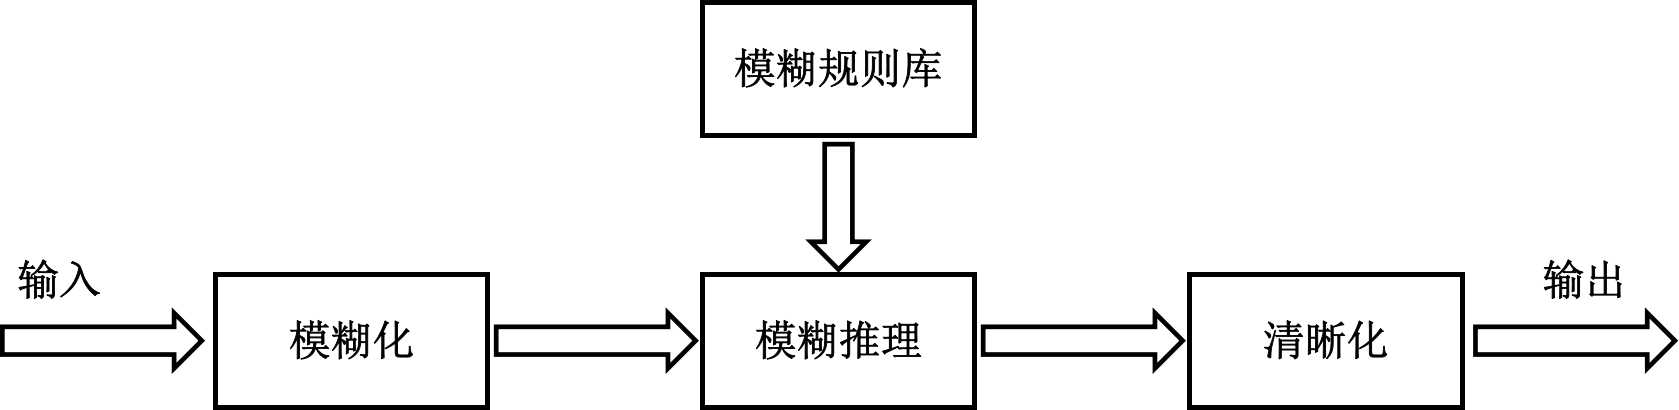
\includegraphics[width=0.8\textwidth]{模糊神经网络的一般性原理流程图.png} % 替换为你的图片文件名
	\caption{模糊神经网络的一般性原理流程图}
	\label{fig:1}
\end{figure}
\par
图~\ref{fig:1}所示为模糊神经网络的一般性原理流程图,一共有四层,分别是:输入层,模糊化层,模糊推理
层,去模糊化层(输出层)。在这个过程中,第一步是模型通过模糊隶属函数对输
入层的输入变量进行模糊化处理,然后将得到的模糊后的信息在模糊推理层中通过模
糊规则库里的规则将其进行组合与推理,最后对模糊推理的输出结果进行去模糊化处
理,得到最终的模型输出。从模糊神经网络模型的整个流程可以看出,对于不同的模
糊神经网络,其主要区别就在于:1、模糊化层使用的模糊隶属函数不同;2、构建的
模糊规则库不一样;此外,关于输入输出方式以及结构层次的选取也会对模糊神经网
络模型有所影响。
\par

\subsection{基于T-S推理的模糊神经网络在语音任务上的应用}

模糊推理系统有着各种各样模糊推理机理,而这其中最常用的有四种:Mamdani
推理,Laresen推理,Tsukamoto推理,Takagi-Sugeno推理[59]。本章将会使用到基于
Takagi-Sugeno(T-S)推理的模糊神经网络模型来研究如何对伪造语音和真实语音进行识别分类。
然而,假如直接使用T-S模型来对语音信号进行鉴伪识别,会出现两个非常严重的问
题:第一是如果T-S模糊神经网络模型的输入数据的维数过大时,会在模糊推理层
出现推理结果普遍无限接近于零的现象,导致整个网络失效;第二是网络中的规则数
是以输入数据的维数作为指数幂的,随着输入数据维数的不断增加,整个网络的规则
数将会呈现指数级增长,形成规则灾难。因为上述两个问题的存在,在伪造语音检测
领域使用模糊神经网络进行分类识别,需要对模糊神经网络的模糊推理过程进行针对
性的调整。文献[58]在使用T-S模糊神经网络进行语音识别就遭遇到上述问题,并提
出使用减法聚类[60]对样本点进行聚类个数的计算来决定模糊推理中规则数的选取,以
及在T-S推理中引入推理补偿因子来避免网络失效,这种解决方案可以借鉴到语音鉴伪上去。文献[27]在上面方法的基础上将减法聚类方法替换成更高效的非均匀数
据规约减法聚类。

\subsection{自适应神经模糊推理系统}
对于模糊神经网络模型,最常用到的一个是自适应神经模糊推理系统[61](Adaptive
Neuro Fuzzy Inference System,ANFIS),它由Jang Roger于1993年提出的一个模糊
神经网络模型,拥有五层结构,是基于T-S推理实现的。ANFIS的模糊推理规则是网
络自动生成的,生成的标准是根据网络输入输出之间的关系。ANFIS的正向传播过程
和普通神经网络一样,以前馈方式传递信息给后面的网络层。
\par
首先对ANFIS的推理规则进行介绍,对于给定的两个输入$x,y$以及一个输出$f$,
基于T-S推理的ANFIS的“if-then”模糊规则如下:
$$if \; x \; is \; A_1 \; and \; y \; is \; B_1, then \; f_1=p_1x+q_1y+r_1$$
式中,$p1, q1, r1$是模糊规则的后件参数。
\par
如图~\ref{fig:2},ANFIS具有输入输出层除外的五层结构,分别是
\par
\begin{figure}[htbp] % htbp 代表 here, top, bottom, page
	\centering
	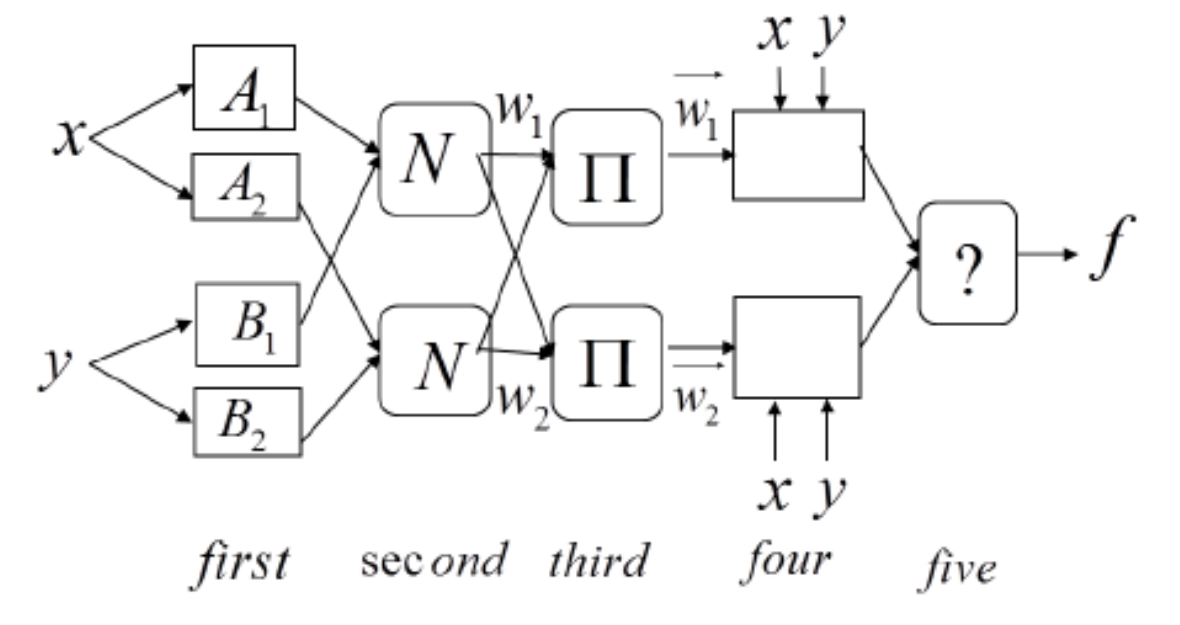
\includegraphics[width=0.6\textwidth]{典型的ANFIS结构.png} % 替换为你的图片文件名
	\caption{典型的ANFIS结构}
	\label{fig:2}
\end{figure}
\par
(1)模糊化层,该层的节点对模糊推理系统的输入变量进行模糊化,这一过程求得每个节点的隶属度函数如下所示
\[O_{\text{i}}^{\text{1}} = \mu_{A_i}(x) \quad i=1,2,\ldots,m \]
式中,节点$A_i$表示模糊子集, $O_{\text{i}}^{\text{1}}$是$x$对$A_i$的隶属度,它确定了输入样本$x$属于$A_i$的程度。
$m$是模糊隶属函数的个数。隶属函数$\mu(x)$的参数需要不断学习得到,这些参数称为前件
参数,前件参数的值不断调整优化会改变ANFIS的推理。
\par
(2)模糊推理层,该层每个的节点代表一条模糊推理规则,对将上一层的隶属
度进行相乘得到结果作为该条规则的触发强度,表达式如下
\[O_{\text{i}}^{\text{2}} = \omega_i = \mu_{A_i}(x)\mu_{B_i}(y) \quad i=1,2,\ldots,m \]
$m$个隶属函数与每一个输入变量相连,在本例子中,输入变量共有2个,那么一共会形
成$m^2$条模糊规则。
\par
(3)第三层的节点数量和第二层一致,该层的节点代表的是模糊规则触发强度进行归一
化之后的值如下:
\[O_{\text{i}}^{\text{3}} = \bar{\omega_i} = \frac{\omega_i}{\sum_j \omega_j} \]
\par
(4)第四层运用上了模糊规则的后件部分并使用它对第三层的模糊规则触发强度进行
加权处理如下:
\[O_{\text{i}}^{\text{4}} = \bar{\omega_i} f_i = \bar{\omega_i} (p_i x + q_i y + r_i) \]
\par
(5)第五层将第四层的输出结果进行求和从而得到系统的总输出
\[O_{\text{i}}^{\text{5}} = \sum{\bar{\omega_i} f_i} = \frac{\sum{\omega_i f_i}}{\sum{\omega_i}} \]
对于上述过程中前件参数和后件参数的学习调整,使用的是最小二乘法以及梯度下
降的误差反向传播(BP算法)相结合的混合算法。训练过程如下:在对后件参数进行
训练调整时,使用的是最小二乘法,在处理这一阶段的参数时,整个网络的前件参数部
分是固定不动的;在调整了后件参数之后,将其保持固定不变,使用误差反向传播算法
对前件参数进行迭代调优。通过上述训练步骤的迭代进行,最终使得ANFIS的前后件参数达到全局最优[62],模型训练完毕。
\par


\section{个人研究方向——深度伪造语音检测}

\subsection{语音深度伪造}
语音深度伪造(Voice Deepfake)是一种基于人工智能技术的手段,它能够通过深度学习算法对原始语音进行高度逼真的模仿和篡改。
这种技术可以生成几乎无法用肉耳分辨的假语音,使得伪造的声音听起来就像是由目标人物亲口说出的一样。
随着深度学习模型的进步,尤其是生成对抗网络(GANs)和其他序列到序列(seq2seq)模型的应用,语音深度伪造的精度和自然度不断提高。
这项技术在某些合法应用中可能有用,例如语音合成、个性化语音助手或者娱乐业,但同时也带来了严重的安全风险和社会问题。
不法分子可能会利用语音深度伪造技术来进行诈骗、身份冒充、操纵信息或实施其他恶意行为,如假冒企业领导发布指示、模仿政府官员传达虚假指令等。
为了应对这一挑战,研究者们正致力于开发反深度伪造技术(语音反欺骗技术),用于检测并鉴别真实与伪造的语音内容。

\subsection{伪造语音检测的难点}
语音深度伪造检测的难点主要包括以下几个方面:
\par
(1)高度真实性和多样性:随着深度学习技术的进步,伪造的语音能够达到非常高的逼真度,甚至可以模拟说话者的情绪、语调和特定口音,这给检测带来了极大挑战。
\par
(2)复杂伪造手段:伪造过程可能涉及复杂的音频处理技术,如多源融合、超分辨率重建等,使得伪造后的语音信号在频谱、时域特征上难以区分。
\par
(3)动态变化性:语音具有很强的个体差异性和情境相关性,同一个人在不同情境下的声音也会有所不同,这要求检测模型具有较强的泛化能力。
\par
(4)缺乏通用特征:尚未发现一种适用于所有情况的稳定声纹特征或深度伪造痕迹,因此需要不断开发和优化用于识别伪造的声学特征提取方法。
\par
(5)对抗攻击:伪造者可能会利用对抗样本生成技术有意地制造难以被现有检测系统识破的伪造语音。
\par
(6)数据依赖性强:构建有效的语音伪造检测系统通常需要大量的真实语音和伪造语音样本进行训练,而高质量的数据集往往不易获取。
\par

\section{基于SAE+FNN的伪造语音检测}
语音合成技术生成的语音对语音特征的影响并不是单一确定的,因此在研究语音鉴伪方法时,
需要考虑语音合成的模糊性,仅仅使用深度学习模型对于语音鉴伪的做法可能稍
有欠缺。考虑到模糊神经网络中的模糊规则推理可以处理模糊信息,并且模糊神经网络
中具有一个使用隶属函数的模糊化层,因此使用栈式自编码器根据样本
数据训练一个深层模型来作为模糊神经网络中的隶属函数,取代传统的高斯函数或者
sigmoid函数等常用隶属函数,这样构造出来的新模型能够同时具备深度学习模型强大
的特征学习能力和模糊神经网络的模糊推理能力。
\par
引入栈式自编码器作为隶属函数的模糊神经网络,记为SAE-FNN。如图~\ref{fig:3}所示
是该模型的结构图,接下来对其具体步骤进行阐述。
\par
\begin{figure}[htbp] % htbp 代表 here, top, bottom, page
	\centering
	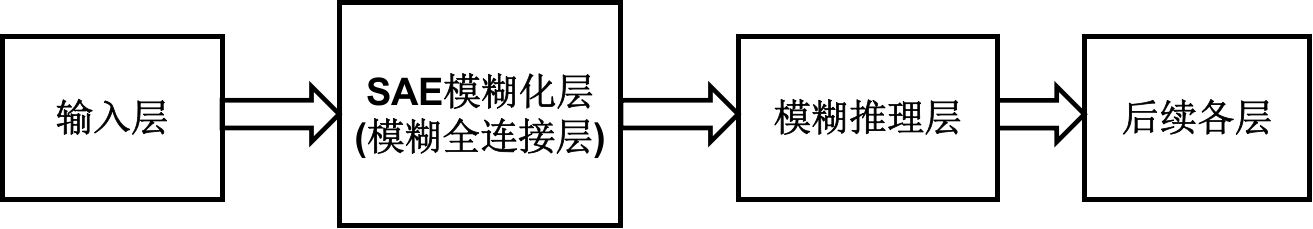
\includegraphics[width=0.8\textwidth]{SAE-FNN模型结构图.png} % 替换为你的图片文件名
	\caption{SAE-FNN模型结构图}
	\label{fig:3}
\end{figure}
\par
第一层是样本输入层,输入的是从语音信号中提取出来的语音特征。
\par
第二层是模糊化层,采用的是一个 SAE 网络结构作为隶属函数,对输入层数据进
行模糊化处理。在这一层,有两个问题需要详细研究:
\par
(1) 该层要用SAE网络作为模糊化层,那么首先要先获得一个SAE网络。如何得
到SAE,在本模型中的做法是使用数据集中所有训练样本直接训练一个SAE模型,并
且进行微调使得SAE模型具有良好的分类性能从而提升该SAE模型作为隶属函数时对
输入向量的模糊化效果。
\par
(2) 本模型因为后面还有一个模糊推理层,所以在这一层中SAE网络对于输入层向
量的处理方式和传统神经网络的处理是不一样的。传统的神经网络对于一个$m$分类问题
中,给定一个输入向量$x(x_1, x_2,\ldots, x_n)$,有$n$个维度,处理方式是直接使用权值矩阵$W$
对$x$进行矩阵运算$W x^T$ ,最终得到相应的一个输出向量$y(y_1, y_2,...,y_m)^T$,向量的每一
个值分别对应着一个类别的归属程度;而在本模型中,输入数据$x(x_1, x_2,\ldots, x_n)$将会被
展开成$n$个数据,每个数据只有一维非零,即$x_{in}={(x_1,0,\ldots,0),(0,x_2,\ldots,0),\ldots,(0,0,\ldots,x_n)}$,
使用权值矩阵$W$进行计算,最终会得到$n$个输出向量$y_{out}=y_{out}^{1},y_{out}^{2},\ldots,y_{out}^{n}$,
其中每一个$y_{out}^{i}$是一个$m$维向量,分别对应着$m$个类别归属程度,即
$y_{out}^{i}=(y_1, y_2,\ldots, y_m), i=1,2,\ldots,n$。
之所以要将输入向量展开,是为了让后续的模糊规则来决定输入向量每一个维度如何组
合来对最终结果的产生贡献。
\par
第三层是模糊推理层,这一层里面的每一个神经元代表一条模糊规则。标准的T-S模糊神经网络模型会出现“维度灾
难”问题。因此本模型采用文献[58]中的办法,使用减法聚类[60]的方式预先对输入数据
维度进行聚类,求得聚类中心的个数作为模糊规则的数量。在模糊推理层中,使用的是
与模糊化层神经元权值连接的方式,权值的大小代表的是相应模糊规则对于模糊推理结
果的贡献程度。
\par
第四层是归一化层,对于上一层的推理结果进行总体的归一化,归一化之后各条模
糊规则的输出结果总和为 1,进行归一化的好处在于可以将后续步骤中网络进行反向调
整参数时,修正的幅度有一个规定的约束范围,避免了网络的大幅度震荡,有助于模糊
神经网络的收敛。
\par
第五层是输出层,将归一化后的各个规则输出结果进行去模糊化,得到输入样本的
分类类别。
\par
上述是的SAE-FNN的前向推理过程。对于反向传播过程,模型里面的各个
参数调整使用反向传播算法,其中需要调整的参数主要有归一化层到输出层之间的权值
参数,模糊化层到模糊推理层之间的权值参数以及隶属函数的参数。
\par
可行性分析:新模型SAE-FNN与传统的模糊神经网络的主要不同之处在于隶属函
数的选择上面以及相应的SAE网络对输入向量的处理方式上面。首先关于隶属函数选
择SAE网络,文献[64,65]指出三层结构使用sigmoid函数作为隐藏层激活函数的BP神
经网络能够任意精度逼近任意连续函数,SAE在网络层次上还要更多,其逼近函数的能
力是可以保证的。此外,关于SAE处理输入向量方式上,在讨论SAE-FNN模型的第二
层结构时,已经展开详细分析了这种方式处理输入向量的具体结果,它有利于后续使用
模糊推理层的模糊规则对上一层的输出进行组合。

\section{基于CNN+FNN的伪造语音检测}
基于CNN+FNN的模糊神经网络模型,这里面的FNN模型使用的是SAE-FNN模
型。语谱图特征具有更优秀的表征语音信息的能力;传统模糊神经网络的输入数据通常是一维的特征向量,当把
模糊神经网络运用于语音鉴伪识别时,它对于高性能的二维语谱图特征无法直接使用,
假如将语谱图从二维数据拉伸扩展成一维向量以适应模糊神经网络的输入规模,那么势
必会破坏语谱图特征在结构上的关联性,影响特征的效果。基于上述两点原因,考虑到
卷积神经网络能处理二维数据,并且具有强大的自动提取特征能力,我们可以将CNN和FNN相结合来对语谱图特征进行语音鉴伪。
\par
\begin{figure}[htbp] % htbp 代表 here, top, bottom, page
	\centering
	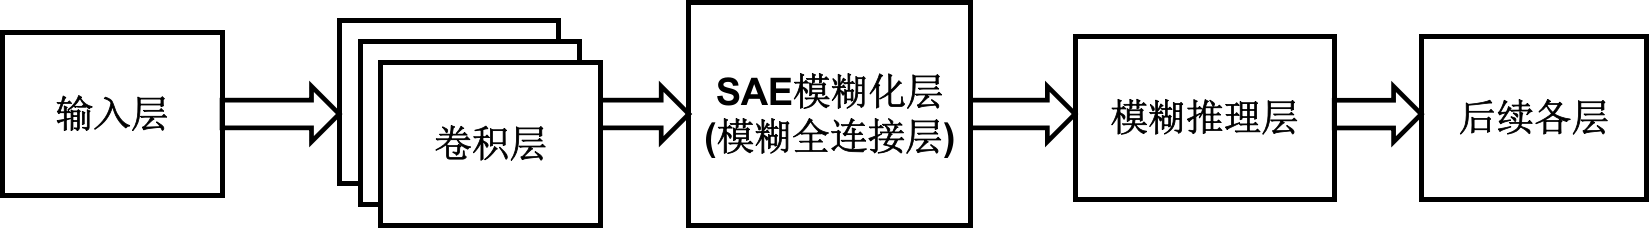
\includegraphics[width=0.8\textwidth]{CNN-FNN模型结构图.png} % 替换为你的图片文件名
	\caption{CNN-FNN模型结构图}
	\label{fig:4}
\end{figure}
\par
\par
如图~\ref{fig:4}所示,CNN-FNN本质上分为两阶段,第一个阶段是使用CNN对二维语谱图进行语音特征提取,
转换成显著性高的一维语音特征向量;第二阶段使用SAE-FNN对第一阶段的特征进行处理。
\par
可行性分析:第一阶段的CNN对二维语谱图特征的提取性能上,由[3]实验结果可以得到验证;
第二阶段的SAE-FNN模型可行性分析在第\ref{sec:1}章已经阐述。所以CNN-FNN模型在理论上是可行的。

\section{结论与思考}
本文深入探讨了基于深度学习和模糊理论的伪造语音检测方法,特别是在构建新型的SAE-FNN模型以及CNN-FNN模型方面进行了理论分析。
SAE-FNN模型利用栈式自编码器作为模糊化层的隶属函数,可以有效地解决传统模糊神经网络在处理高维输入数据时可能出现的“维度灾难”问题,并通过反向传播算法优化模型参数,提高了对伪造语音特征的识别能力。
CNN-FNN模型则结合了卷积神经网络强大的二维数据处理能力和模糊神经网络的模糊推理优势,能针对语谱图特征进行有效提取和分类。理论上,采用CNN-FNN模型对伪造语音检测可以取得比传统方法更优秀的性能,尤其是对于包含丰富语音信息的语谱图特征,该模型能够更好地保持其内在结构关联性,从而提升鉴伪准确率。
\par
通过运用模糊理论知识与个人研究方向结合,论述了的两种融合深度学习与模糊理论的伪造语音检测模型在理论上具有可行性,
显示了深度学习和模糊理论相结合的方法在语音领域的应用具有广阔的研究前景和价值,
对后续的个人研究有较大帮助,开拓了新的思维方式。

% Please add the following required packages to your document preamble:
\usepackage{multirow}
\begin{table}[]
	\begin{tabular}{lllll}
	1                  & 2 & 3 & 4 &  \\
	\multirow{2}{*}{2} &   &   &   &  \\
					   &   &   &   &  \\
					   &   &   &   & 
	\end{tabular}
	\end{table}

\begin{thebibliography}{4}
	\bibitem{Butterworth}Butterworth S. On the theory of filter amplifiers[J]. Wireless Engineer, 1930, 7(6): 536-541.
\end{thebibliography}


\end{document}
